\lstdefinestyle{csharp}{
    language=C#,
    basicstyle=\ttfamily\small,
    commentstyle=\color{green!40!black},
    keywordstyle=\color{blue},
    numberstyle=\tiny\color{gray},
    numbers=left,
    stepnumber=1,
    numbersep=5pt,
    backgroundcolor=\color{white},
    showspaces=false,
    showstringspaces=false,
    showtabs=false,
    tabsize=2,
    frame=single,
    rulecolor=\color{black},
    captionpos=b,
    breaklines=true,
    breakatwhitespace=false,
    title=\lstname,
    escapeinside={\%*}{*)},
    morekeywords={var},
}


\chapter{Feinkonzept und Realisierung}

\section{Entwicklungsumgebungen}
\subsection{Visual Studio 2022}
Visual Studio 2022 ist eine integrierte Entwicklungsumgebung (IDE) von Microsoft, die speziell für die Entwicklung von
Softwareanwendungen, Webanwendungen und Desktop-Anwendungen konzipiert ist. Es handelt sich um eine umfangreiche
Entwicklungsumgebung, die von Entwicklern weltweit für eine breite Palette von Anwendungsfällen eingesetzt wird.

\subsection{Unity Editor}
Der Unity-Editor ist eine leistungsstarke integrierte Entwicklungsumgebung (IDE) und eine zentrale Arbeitsumgebung
für die Erstellung von 2D-, 3D-, Augmented Reality (AR) und Virtual Reality (VR) Anwendungen und Spielen. Er wird von
Unity Technologies entwickelt und ist die Hauptplattform für die Entwicklung von Unity-basierten Projekten.

\subsection{Managers}
In diesem Level werden mehrere von Unity und dem Mixed Reality Toolkit 3 bereits
bereitgestellten Manager \footnote{Medium \cite{Managers}} verwendet. Unter einer Manager
versteht man eine Komponente die einer Unity-Scene hinzugefügt wird die dazu dient,
bestimmte Aspekte oder Funktionen der Anwendung zu verwalten und zu stuern. Diese Manager
spielen eine wichtige Rolle in der Organisation und Kontroller verschiedener Teile der Unity-Anwendung.
In dem "Knappsack Problem Level" werden folgende Manager verwendet:
\begin{itemize}
    \item ARPlaneManager\footnote{Unity \cite{PlaneManager}}:\\
    Dieser Manager wird verwendet um in der Umgebung des Benutzers alle Horizontalen Flächen zu erkennen und zu tracken.
    Außerdem erleichtert er das platzieren von Objekten in der echten Welt.
    Diese Flächen werden anschließend mit einer Textur markiert. Wenn der User für die vorgeschriebene
    Zeit auf eine dieser Flächen schaut wird in der Mitte dieser Fläche das Inventar als 3D Objekt dargestellt. An dieses
    3D Objekt wird anschließend auch ein Spatial Anchor angehängt und in dem ARAnchorManager verwaltet.

    \item ARRaycastManager\footnote{Unity \cite{RaycastManager}}; \\
    Dieser Manager wird verwendet um aus einem Origin Punkt also in diesem Fall die Kamera der HoloLens2, raycasting durchzuführen.
    Diese Raycasts treffen dann auf bereits markierte und getrackte Planes. Wenn dies der Fall ist, ist bekannt, dass der
    Benutzer auf dieses Plane sieht. Dies ermöglicht dann eine akkurate Platzierung eines 3D Objekts in der realen Welt. \\
\end{itemize}

\section{Hauptmenu}
Das Hauptmenu dient dazu um das Basic UI/UX System zu implementieren.
Hier kann der Benutzer dann diverse Einstellungen Tätigen als auch
das gewünschte Level auswählen und starten

\subsection{UI/UX}
Mittels verwendung des UX-Tools-Plug-Ins für Mixed Reality wird
mit bereitgestellten Knöpfen, Oberflächen, Comboboxen, etc...
die Benutzeroberfläche erstellt.

\subsection{Laden der Level}
Durch einen Knopfdruck wird dann in Unreal Engine das der ausgewählte
Level geladen.
%Hier dann noch Bilder vom Code einfügen

\section{Ping Level}
In diesem Level wird das IT-Grundprinzip eines Pings dargestellt.
In einer realen Umgebung sind zwei PCs durch ein
rotes Kabel miteinander verbunden. Der Benutzer trägt die
HoloLens 2 und kann durch Drücken eines Knopfes ein Foto der Umgebung
aufnehmen, anschließend werden dann Raycasts verwendet,
um die genaue Position des roten Kabels in der physischen
Welt zu bestimmen. Durch erneutes Drücken des Knopfes wird
ein virtuelles Ping-Paket erzeugt, das entlang des roten
Kabels hin und her wandert. Dieser Vorgang visualisiert
die Netzwerkverbindung zwischen den beiden PCs.
Der Benutzer kann das Ping-Paket durch die HoloLens 2 verfolgen,
da es die physische Verbindung zwischen den beiden Computern
simuliert. Mit einem weiteren Knopfdruck werden einaml Simplere
und einmal detaillierte Informationen über das Ping-Paket angezeigt.
Angezeigt wird dann die Ziel-Ip-Adresse, Quell-Ip-Adresse, die gesamte länge
 sowie die time to Live. Die Benutzeroberfläche
schwebt virtuell über dem roten Kabel, sodass der Benutzer
die Informationen einfach betrachten kann.

\clearpage

\subsection{Aufbau von Ping Level}
In diesen Abschnitt wird beschrieben wie die Unity Scene aufgebaut ist und
was die aufgabe der einzelnen GameObjects\footnote{Unity \cite{GameObject}} ist.

\subsection{Gameobject}
Ein Unity GameObject ist die grundlegende Einheit in der Unity-Spieleentwicklung
und repräsentiert eine Spielkomponente, die sowohl grafische als auch funktionale
Elemente enthalten kann. Es dient als Container für Komponenten wie Modelle,
Texturen, Skripte und Kollisionsformen, die gemeinsam ein interagieren können.
GameObjects können sowohl 3D- als auch 2D-Objekte sein und ermöglichen die
Realisierung von Spielfiguren, Umgebungen,Effekten und mehr. Durch die
Verknüpfung von GameObjects mit Skripten kann man Verhalten und
Interaktionen programmieren.

\begin{figure}[h]
    \centering
    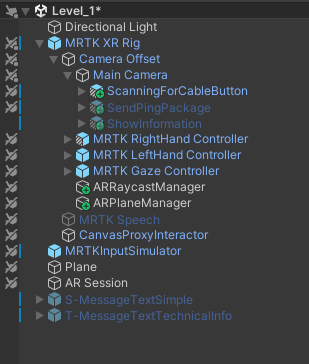
\includegraphics[scale=1]{images/Level1Hierarchy}
    \caption{Hierarchie des Ping Levels im Unity Editor.}
    \label{fig:level1_hierarchy}
\end{figure}
\begin{itemize}
    \item \textbf{level-1:} Die Scene in der Alle Unity-Objekte enthalten sind.
    \item \textbf{ScanningForCable:} Knopf welcher den Prozess zur realisierung der Position des Kabels startet.
    \item \textbf{ShowInformation:} Knopf welcher den Informationen über das virtuelle Ping Paket anzeigt.
    \item \textbf{S-MessageTextSimple:} Simpler Text welcher angezeigt wird sobald ShowInformation Knopf gedrückt wurde.
    \item \textbf{S-MessageTextTechnicalInfo:} gleich wie S-MessageTextSimple nur mit den technischen informationen.
\end{itemize}


\subsection{Object Tracking}
\subsection*{Foto der umgebung schießen}
Nach betätigen des Knopfes am anfang, wird ein Foto von der Umgebung gemacht.
\begin{lstlisting}[style=csharp, caption={}, label=code:takingPicture]
void takingPicture()
{
    if (!takingNewPicture)
    {
        redPixelCoordinates.Clear();
        takingNewPicture = true;

        PhotoCapture.CreateAsync(false, delegate (PhotoCapture captureObject)
        {
            if (captureObject != null)
            {
                photoCaptureObject = captureObject;
                CameraParameters cameraParameters = new CameraParameters();
                cameraParameters.hologramOpacity = 0.0f;
                cameraParameters.cameraResolutionWidth = cameraResolution.width;
                cameraParameters.cameraResolutionHeight = cameraResolution.height;
                cameraParameters.pixelFormat = CapturePixelFormat.BGRA32;
                try
                {
                    photoCaptureObject.StartPhotoModeAsync(cameraParameters, delegate (PhotoCapture.PhotoCaptureResult result)
                    {
                        photoCaptureObject.TakePhotoAsync(onCapturedPhotoToMemory);
                    });
                }
                catch (Exception e)
                {
                    Debug.LogWarning(e);
                }
            }
        });
    }
}
\end{lstlisting}
\textbf{Erklärung:}
\begin{enumerate}
    \item \textbf{redPixelCoordinates:} Ist eine List<Vector2> welche hier geleert wird und wo später die x und y coordinaten der roten Pixel gespeichert werden.
    \item \textbf{cameraParameters:} Ein Parameter, der Einstellungen für die Kamera festlegt. cameraParameter ist ein Objekt des Typs CameraParameters, das in Unity für die Konfiguration von Kameraeigenschaften verwendet wird, wenn mit der PhotoCapture-API gearbeitet wird.
    \item \textbf{photoCaptureObject.StartPhotoModeAsync:} Die Funktion startet den Fotoaufnahmemodus der Kamera asynchron. Der cameraParameters-Parameter enthält Einstellungen für die Kamera, und der delegate-Block wird aufgerufen, wenn der Fotoaufnahmemodus gestartet wurde.
    \item \textbf{photoCaptureObject.TakePhotoAsync(onCapturedPhotoToMemory):} Dieser Befehl löst das eigentliche Aufnehmen des Fotos aus. Das Foto wird dann an die Methode onCapturedPhotoToMemory übergeben, wenn die Aufnahme abgeschlossen ist.\\
\end{enumerate}


\subsection*{Foto der umgebung schießen}
Nach betätigen des Knopfes am anfang, wird ein Foto von der Umgebung gemacht.
\begin{lstlisting}[style=csharp, caption={}, label=code:onCapturedPhotoToMemory]
void onCapturedPhotoToMemory(PhotoCapture.PhotoCaptureResult result, PhotoCaptureFrame photoCaptureFrame)
    {
        photoCaptureFrame.UploadImageDataToTexture(targetTexture);

        editTexture(targetTexture);

        photoCaptureObject.StopPhotoModeAsync(onStoppedPhotoMode);
    }
\end{lstlisting}
\textbf{Erklärung:}
\begin{enumerate}
    \item \textbf{photoCaptureFrame.UploadImageDataToTexture:} Kopiert das unverarbeitete Foto in die globale variable targetTexture. targetTexture ist ein Texture2D\footnote{Unity \cite{Texture2D}} Klasse welches für texturen in C# Programme benutzt wird.
    \item \textbf{editedTexture:} Diese Funktion bearbeitet das Foto und sucht nach roten Pixeln.
    \item \textbf{photoCaptureObject.StopPhotoModeAsync(onStoppedPhotoMode):} Beendet die instanz des Photocapture und ruft dannach die funktion onStoppedPhotoMode.
\end{enumerate}




\subsection{Kurvenberechnung}
Durch Berechnung der Kurve wird das Kabel als Kurve gespeichert
und dadurch wird es ermöglicht, dass das 3D-Ping-Paket über diese
Kurve von einem PC zum anderen läuft.
% Hier dann noch Code zur Kurvenberechnung einfügen


\section{Knapsack Problem Level}
Im zweiten Level dieses Projekts steht das Knapsack-Problem im Fokus.
Ziel ist es, einen Programmieralgorithmus mithilfe von Augmented Reality
(AR) darzustellen. Dieser Algorithmus wird nicht nur in der Höheren
Technischen Lehranstalt (HTL) vermittelt, sondern die Benutzer sollen
ihn auch selbst programmieren können.

Der Level beginnt damit, dass der Benutzer aufgefordert wird, auf eine
horizontale, flache Oberfläche zu schauen. Diese Oberfläche kann ein Tisch,
der Boden oder ähnliches sein. Der Benutzer wird dann gebeten, für eine bestimmte
vorgegebene Zeit auf diese Oberfläche zu schauen. Nach dieser Zeit werden das Inventar,
der Solve-Button und drei Informationslabels auf dieser Oberfläche platziert.

Das Inventar wird durch ein 3x3 zweidimensionales Gitter repräsentiert, ähnlich
wie das Inventar in einem Spiel. Zusätzlich befinden sich auf der Oberfläche 11 Bauklötze,
die mit QR-Codes versehen sind. Diese Bauklötze repräsentieren die Items, die der Benutzer
in das Inventar legen kann. Durch Aufheben und Nahheranhalten an die HoloLens wird der QR-Code gescannt.
Dadurch werden das dazugehörige 3D-Modell, der Wert und das Gewicht des Items angezeigt.
Diese Informationen sind für den Benutzer wichtig, um das Gewicht des Items und
seinen Einfluss auf das Inventar zu verstehen.

Nach dem Scannen kann der Benutzer einen beliebigen Bauklotz in das Inventar platzieren.
Wenn der Benutzer wissen möchte, welchen Wert seine Lösung hat, kann er auf den Solve-Button
klicken. Dies löst den Knapsack-Algorithmus aus, der den Wert des eigenen Inventars berechnet.
Zusätzlich wird die optimale Lösung für das Problem ermittelt.

Insgesamt bietet dieses Unity Level für die HoloLens 2 eine interaktive und visuelle Erfahrung,
bei der die Benutzer das Knapsack-Problem nicht nur verstehen, sondern auch praktisch anwenden können.

\subsection{Aufbau von dem Knapsack-Problem Level}
In diesem Abschnitt wird darauf eingegangen wie das Knapsack-Problem Level im Unity Editor aufgebaut ist.
Zusätzlich wird erklärt was genau auf diesem Bild dargestellt wird und wie es funktioniert.\\

\begin{figure}[h]
    \centering
    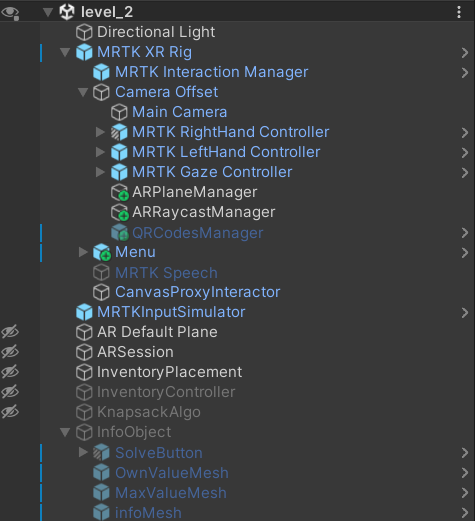
\includegraphics[scale=0.8]{images/Level2Hirarchy}
    \caption{Hierarchie des Knapsack-Problem Levels im Unity Editor.}
    \label{fig:level2_hierarchy}
\end{figure}

In dieser Abbildung wird der Aufbau der Scene\footnote{Unity \cite{Scene}} von dem Knapsack-Problem Level dargestellt.
Zu sehen ist auf diese Abbildung folgendes:
\begin{itemize}
    \item \textbf{level-2:} Die Scene in der Alle Unity-Objekte enthalten sind.
    \item \textbf{MRTK XR Rig:} Das Objekt in dem die Hauptkomponenten wie z.B.: \textit{Main Camera, MRTK Interaction Manager, Alle Manager, etc... } für die AR-Applikation enthalten sind.
    \item \textbf{AR Default Plane:} Ein Objekt das auf große Flächen verweißt und diese mit hilfe des ARPlaneManagers markiert.
    \item \textbf{ARSession:} Objekt, dass sich um eine Laufzeitumgebung oder einen Kontext, der für die Erfassung, Verarbeitung und Darstellung von AR-Inhalten kümmert.
    \item \textbf{InventoryPlacement:} Objekt dem das selbstgeschriebene \textit{Anchorscript} zugewiesen ist, dass sich um das platzieren des Inventars kümmert.
    \item \textbf{InventoryController:} Objekt, dass sich Frame für Frame überprüft ob ein neues Item in das Inventar hinzugefügt wurde.
    \item \textbf{KnapsackAlgo:} Ist das Objekt, dem das KnapsackAlgorithmus Script zugewiesen ist und sich darum kümmert, dass das \textit{Momentane Inventar, der Maximale mögliche Wert und die perfekte Lösung} berechnet werden.
    \item \textbf{InfoObject:} Ist eine Sammlung an 3D-Objekten um das KnapsackAlgorithmusScript auszuführen und die errechneten Werte darzustellen.\\
\end{itemize}

Wenn der Name eines Objekts wie in der Abbildung sichtbar ausgegraut ist, heißt das, dass das Objekt zu Programmstart deaktiviert ist und daher nicht ausgeführt wird.
Wenn neben dem Objekt ein durchgestrichenes Auge sichtbar ist, bedeuted das, dass das Objekt in der Unity Scene nicht sichtbar aber aktiviert ist und daher zu Programmstart direkt gestartet wird.

\subsection{QR-Code Tagging}
Generierte QR-Codes werden auf die realen Objekte geklebt. In diesen QR-Codes werden
wichtige Informationen zu den Objekten gespeichert. Darunten sind folgende Elemente:
Gewicht, Wert und eine kurze Beschreibung zu diesem Objekt.

\subsection{QR-Code Tracking}
Durch Verwendung der integrierten Kamera rendert die HoloLens2 existente QR-Codes an
der Originalen Positionen in 3D-Objekte. Mittels tracking kann dann auch der Inhalt
der getracked QR-Codes geladen werden.
%Genauer Beschreibung + wenn vorhanden Code und Blueprints von QR-Code-Tracking hinzufügen

\subsection{Platzieren des Inventars}
In dem folgendem Abschnitt wird die PlaceObjectOnLookedAtDesk Klasse der AARiE Applikation beschrieben, die das platzieren des Inventars,
Solve Buttons, und Info-Mehes implementiert.

\subsection*{Frame-Aktualisierung um richtiges Plane zu finden}
\begin{lstlisting}[style=csharp, caption={}, label=code:update]
void Update()
{
    if (!objectPlaced && canStartScript)
    {
        List<ARRaycastHit> hits = new List<ARRaycastHit>();
        // Use Camera.main.transform.forward as the ray direction
        if (raycastManager.Raycast(new Ray(Camera.main.transform.position, Camera.main.transform.forward), hits, TrackableType.Planes))
        {
            ARPlane closestPlane = FindClosestPlane(hits);
            if (closestPlane != null)
            {
                if (selectedDeskPlane == null || selectedDeskPlane != closestPlane)
                {
                    selectedDeskPlane = closestPlane;
                    lookStartTime = Time.time; // Start the timer when a new plane is selected.
                }
                float timeLookedAtPlane = Time.time - lookStartTime;
                if (timeLookedAtPlane >= requiredLookTime)
                {
                    PlaceObjectOnDesk(selectedDeskPlane);
                    objectPlaced = true;
                }
            }
            else
            {
                selectedDeskPlane = null;
            }
        }
        else
        {
            selectedDeskPlane = null;
        }
    }
}
\end{lstlisting}
\textbf{Erklärung:}
\begin{enumerate}
    \item \textbf{Bedingte Aktualisierung:} Die Update-Funktion wird nur ausgeführt, wenn das Objekt noch nicht platziert wurde und das Skript gestartet werden kann. Wenn die Funktion dann gestartet wird, wird diese jeden Frame 1 mal ausgeführt.
    \item \textbf{Raycasting auf Planes:} Ein Raycast wird durchgeführt, um festzustellen, ob die Kamera auf ein AR-Plane blickt.
    \item \textbf{Suche nach dem nächsten AR-Plane:} Die Funktion \texttt{FindClosestPlane} wird aufgerufen, um das nächste AR-Plane zu finden.
    \item \textbf{Zeiterfassung für Blickzeit:} Die Zeit, die auf das ausgewählte AR-Plane geschaut wurde, wird gemessen.
    \item \textbf{Platzierung des Objekts bei ausreichender Blickzeit:} Wenn die benötigte Blickzeit überschritten wurde, wird die Funktion \texttt{PlaceObjectOnDesk} aufgerufen und das Objekt wird platziert.\\
\end{enumerate}

\subsection*{Das am kürzesten entfernte Plane\footnote{Unity \cite{Plane}} finden}
\begin{lstlisting}[style=csharp, caption={}, label=code:findclosestplane]
ARPlane FindClosestPlane(List<ARRaycastHit> hits)
{
    ARPlane closestPlane = null;
    float closestDistance = float.MaxValue;
    foreach (var hit in hits)
    {
        ARPlane plane = planeManager.GetPlane(hit.trackableId);
        if (plane != null)
        {
            float distanceToPlane = Vector3.Distance(Camera.main.transform.position, hit.pose.position);
            if (distanceToPlane < closestDistance)
            {
                closestPlane = plane;
                closestDistance = distanceToPlane;
            }
        }
    }
    return closestPlane;
}
\end{lstlisting}

\textbf{Erklärung:}
\begin{enumerate}
    \item \textbf{Suche nach der nächsten AR-Plane:} Die Funktion durchläuft alle getroffenen AR-Planes und findet diejenige mit der geringsten Distanz zur Kamera.
    \item \textbf{Berechnung der Distanz:} Die Distanz zwischen der Kameraposition und der Position der getroffenen AR-Plane wird berechnet.
    \item \textbf{Vergleich der Distanzen:} Die Distanz zur aktuellen AR-Plane wird mit der bisher geringsten Distanz verglichen. Wenn sie kleiner ist, wird die aktuelle AR-Plane als nächste ausgewählt.\\
\end{enumerate}

\subsection*{Berechnung der Position und aktivierung/deaktivierung sämtlicher Objekte}
\begin{lstlisting}[style=csharp, caption={}, label=code:placeobject]
void PlaceObjectOnDesk(ARPlane deskPlane)
{
    qrCodesManager.SetActive(true);
    // Calculate the object's position above the center of the plane.
    Vector3 objectPosition = deskPlane.center + Vector3.up * heightOffset;
    // Calculate the rotation to rotate the object -90 degrees around the x-axis.
    Quaternion objectRotation = Quaternion.Euler(-90f, 0f, 0f);
    // Instantiate the object with rotation.
    GameObject instantiatedObject = Instantiate(inventoryObject, objectPosition, objectRotation);
    // Set the scale of the instantiated object.
    instantiatedObject.transform.localScale = new Vector3(20f, 20f, 20f);
    // Spawn infoGameObject (Two TextMeshes and button for Knapsack Algorithm)
    Vector3 infoObjectPosition = objectPosition - Vector3.forward * 4.415f + Vector3.right * 0.4f;
    infoObject.transform.position = infoObjectPosition;
    infoObject.SetActive(true);
    // Set the inventoryObject in the InventoryController
    inventoryController.SetInventoryObject(instantiatedObject);
    // Enable the InventoryController
    inventoryController.gameObject.SetActive(true);
    // Set the visibility of the planes.
    planeManager.planePrefab.SetActive(false);
    // Disable this script so it won't run again.
    gameObject.SetActive(false);
}
\end{lstlisting}

\textbf{Erklärung:}
\begin{enumerate}
    \item \textbf{Aktivierung von QR-Codes und Objektplatzierung:} Die QR-Code-Manager werden aktiviert, und die Position des zu platzierenden Objekts wird berechnet.
    \item \textbf{Berechnung der Objektposition und Rotation:} Die Position des Objekts wird über dem Zentrum der ausgewählten AR-Plane berechnet, und die Rotation wird auf -90 Grad um die x-Achse festgelegt.
    \item \textbf{Instantiierung des Objekts:} Das Objekt wird instanziiert und skaliert.
    \item \textbf{Platzierung des infoGameObject:} Die Position des Info-Objekts (TextMeshes und Button für den Knapsack-Algorithmus) wird festgelegt und aktiviert.
    \item \textbf{Setzen des Inventarobjekts im InventoryController:} Das platzierte Objekt wird im InventoryController festgelegt.
    \item \textbf{Aktivierung des InventoryController:} Der InventoryController wird aktiviert.
    \item \textbf{Sichtbarkeit der Planes ausschalten:} Die Sichtbarkeit der AR-Planes wird ausgeschaltet.
    \item \textbf{Deaktivierung des Skripts:} Das aktuelle Skript wird deaktiviert, damit es nicht erneut ausgeführt wird.\\
\end{enumerate}

\subsection{Inventar-Controller}
In diesem Abschnitt wird genauer auf das InventarController Script eingegangen und erklärt wie dieses funktioniert.

%Hier Code einfügen hihi

\subsection{Knappsack-Algorithmus}
In dem folgendem Abschnitt wird auf die Funktion \texit{KnapsackMaxValue} des \texit{KnapsackScript.cs} eingegangen, die den Knapsack-Algorithmus
implementiert. Diese Funktion errechnet sich den Maximal-erreichbaren Wert und die perfekte Lösung.

\subsection*{Funktionsaufruf}
\begin{lstlisting}[style=csharp, caption={}, label=code:init]
int maxValue = KnapsackMaxValue(out usedItems, out int coveredCapacity);
int inventoryValue = -1;
maxMesh.text = "Maximal erreichbarer Wert: " + maxValue.ToString();
\end{lstlisting}
\textbf{Erklärung:} Hier wird die Funktion aufgerufen und dem textMesh \textbf{maxMesh} wird dieser Wert zugewiesen um dem User diesen Wert darzustellen.\\

\subsection*{Variablen Initialisierung}
\begin{lstlisting}[style=csharp, caption={}, label=code:variable]
int n = items.Count;
int[,] dp = new int[n + 1, capacity + 1];
bool[,] selected = new bool[n + 1, capacity + 1];
\end{lstlisting}
\textbf{Erklärung:} Die Initialisierung erstellt die notwendigen Arrays für die dynamische Programmierung.\\

\subsection*{Knapsack-Algorithmus}
\begin{lstlisting}[style=csharp, caption={}, label=code:dynamic]
for (int i = 0; i <= n; i++)
{
    for (int w = 0; w <= capacity; w++)
    {
        // Initialisierung der DP-Tabelle
        if (i == 0 || w == 0)
            dp[i, w] = 0;
        else if (items[i].weight <= w && i <= maxItems)
        {
            // Berechnung des neuen Werts, wenn das Item ausgewählt wird
            int newValue = items[i].value + dp[i - 1, w - items[i].weight];
            if (newValue > dp[i - 1, w])
            {
                dp[i, w] = newValue;
                selected[i, w] = true;
            }
            else
            {
                dp[i, w] = dp[i - 1, w];
                selected[i, w] = false;
            }
        }
        else
        {
            dp[i, w] = dp[i - 1, w];
            selected[i, w] = false;
        }
    }
}
\end{lstlisting}

\textbf{Erklärung:}
\begin{enumerate}
    \item \textbf{Iterationen durch die Items und Kapazität:} Die äußere Schleife durchläuft jedes Item (\texttt{i}) von 0 bis zur Gesamtanzahl der Items (\texttt{n}). Die innere Schleife durchläuft jede mögliche Kapazität (\texttt{w}) von 0 bis zur maximalen Kapazität des Rucksacks.

    \item \textbf{Initialisierung der DP-Tabelle:} Wenn \texttt{i} oder \texttt{w} 0 ist, wird der Wert in der DP-Tabelle auf 0 gesetzt. Dies liegt daran, dass es keine Items gibt oder die Kapazität des Rucksacks 0 ist.

    \item \textbf{Überprüfung, ob das Item ausgewählt werden kann:} Wenn das aktuelle Item ausgewählt werden kann (basierend auf Gewicht und maximaler Anzahl von Items), wird der neue Wert berechnet, wenn das Item ausgewählt wird.

    \item \textbf{Vergleich und Auswahl:} Der neue Wert wird mit dem Wert verglichen, wenn das Item nicht ausgewählt wird. Wenn der neue Wert größer ist, wird das Item ausgewählt (\texttt{selected[i, w] = true}), andernfalls wird das vorherige Ergebnis beibehalten (\texttt{selected[i, w] = false}).

    \item \textbf{Falls Item nicht ausgewählt wird:} Wenn das aktuelle Item nicht ausgewählt wird, wird der Wert in der DP-Tabelle auf den Wert gesetzt, den das Rucksack ohne das aktuelle Item in der vorherigen Iteration erreicht hat.\\
\end{enumerate}

\subsection*{Backtracking, um ausgewählte Items und perfekt Lösung zu finden}
\begin{lstlisting}[style=csharp, caption={}, label=code:backtrack]
List<List<int>> tempUsedItems = new List<List<int>>();
int row = n;
int col = capacity;
while (row > 0 && col > 0)
{
    List<int> group = new List<int>();
    while (row > 0 && col > 0 && selected[row, col])
    {
        // Item zu ausgewählter Gruppe hinzufügen
        group.Add(items[row].id);
        col -= items[row].weight;
        row--;
    }

    // Hinzufügen der Gruppe zur Liste
    if (group.Count > 0)
    {
        tempUsedItems.Add(group);
    }

    // Fortfahren mit dem Backtracking
    if (row > 0 && col > 0)
    {
        row--;
    }
}
\end{lstlisting}

\textbf{Erklärung:}
\begin{enumerate}
    \item \textbf{Initialisierung von Zeilen- und Spaltenindizes:} Die Variablen \texttt{row} und \texttt{col} werden auf die letzte Zeile und Spalte der DP-Tabelle gesetzt.

    \item \textbf{Hauptschleife für Backtracking:} Die äußere Schleife wird durchlaufen, solange die Zeile und die Spalte größer als 0 sind.

    \item \textbf{Innere Schleife für Gruppenbildung:} Solange die Zeile und die Spalte größer als 0 sind und das Item in der DP-Tabelle ausgewählt wurde (\texttt{selected[row, col]}), wird das Item zur aktuellen Gruppe hinzugefügt, das Gewicht von der aktuellen Kapazität abgezogen, und die Zeile wird dekrementiert.

    \item \textbf{Hinzufügen der Gruppe zur Liste:} Wenn die Gruppe mindestens ein Item enthält, wird die Gruppe zur temporären Liste \texttt{tempUsedItems} hinzugefügt.

    \item \textbf{Fortfahren mit dem Backtracking:} Die Zeile wird dekrementiert, um das nächste ausgewählte Item zu finden.
\end{enumerate}

Diese Schritte werden wiederholt, bis alle ausgewählten Items gefunden sind und die temporäre Liste \texttt{tempUsedItems} alle ausgewählten Gruppen enthält.\\

\subsection*{Gruppengröße berechnen}
\begin{lstlisting}[style=csharp, caption={}, label=code:maxgroup]
int maxGroupSize = 0;
foreach (var group in tempUsedItems)
{
    if (group.Count > maxGroupSize)
        maxGroupSize = group.Count;
}
\end{lstlisting}
\textbf{Erklärung:} Findet die maximale Gruppengröße.\\

\subsection*{Temporäres Array umwandeln und das usedItems Array befüllen}
\begin{lstlisting}[style=csharp, caption={}, label=code:convert]
usedItems = new int[tempUsedItems.Count, maxGroupSize];
for (int i = 0; i < tempUsedItems.Count; i++)
{
    for (int j = 0; j < tempUsedItems[i].Count; j++)
    {
        usedItems[i, j] = tempUsedItems[i][j];
    }
}
\end{lstlisting}
\textbf{Erklärung:} Konvertiert die temporäre Liste von Gruppen in ein 2D-Array, um die ausgewählten Items also die perfekt Lösung zu speichern.\\

\subsection*{Rückgabewert}
\begin{lstlisting}[style=csharp, caption={}, label=code:return]
return dp[n, capacity];
\end{lstlisting}
\textbf{Erklärung:} Gibt den Gesamtwert des besten Rucksacks zurück.\\

\subsection{Berechnen des eigenen Inventars}
In diesem Abschnitt wird auf die Funktion \textit{KnapsackInventoryValue} des \texit{KnapsackScript.cs} eingegangen. Diese Funktion
berechnet das Inventar Value des selbst gebauten Inventars.

\subsection*{Funktionsaufruf}
\begin{lstlisting}[style=csharp, caption={}, label=code:aufruf]
inventoryValue = KnapsackInventoryValue(inventory);
if (maxValue == inventoryValue)
{
    infoMesh.color = Color.green;
    infoMesh.text = "Maximale Punktzahl erreicht";
}
else
{
    infoMesh.text = "";
}
ownMesh.text = "Erreichter Wert: " + inventoryValue.ToString();
\end{lstlisting}
\textbf{Erklärung:}
\begin{enumerate}
    \item \textbf{Inventar Wert berechnen:} Die Funktion KnapsackInventoryValue wird mit dem übergebenem invetory aufgerufen und der Inventar Wert berechnet.
    \item \textbf{Ergebnis Handling:} Wenn der eigene Wert gleich dem Maximalen errechnetem Wert enspricht hat der Benutzer gewonnen. Anderenfalls wird dem \texit{infoMesh} der aktuelle Wert zugewiesen.
\end{enumerate}

\subsection*{Code für die Berechnung des eigenen Inventars}
\begin{lstlisting}[style=csharp, caption={}, label=code:ownInventory]
int KnapsackInventoryValue(int[,] inventory)
{
    if(inventory == null)
    {
        throw new System.Exception("Inventory is null");
    }

    int totalValue = 0;

    foreach (var item in items.Values)
    {
        int itemId = item.id;
        int itemValue = item.value;

        for (int j = 0; j < inventory.GetLength(0); j++)
        {
            for (int k = 0; k < inventory.GetLength(1); k++)
            {
                if (inventory[j, k] == itemId)
                {
                    totalValue += itemValue;
                }
            }
        }
    }

    return totalValue;
}
\end{lstlisting}
\textbf{Erklärung:}
\begin{enumerate}
    \item \textbf{Überprüfung auf Null:} Die Funktion überprüft, ob das übergebene Inventar null ist. Falls ja, wird eine Ausnahme ausgelöst.

    \item \textbf{Initialisierung des Gesamtwerts:} Die Variable \texttt{totalValue} wird auf 0 initialisiert. Hier wird der Gesamtwert des Rucksackinventars gespeichert.

    \item \textbf{Durchlauf aller Gegenstände:} Die Funktion durchläuft alle Gegenstände im globalen \texttt{items}-Dictionary.

    \item \textbf{Extrahierung von Informationen:} Für jeden Gegenstand werden die ID (\texttt{itemId}) und der Wert (\texttt{itemValue}) extrahiert.

    \item \textbf{Durchlauf des Inventars:} Die doppelte Schleife durchläuft das gesamte Inventar (\texttt{inventory}) und prüft, ob der aktuelle Gegenstand vorhanden ist.

    \item \textbf{Berechnung des Gesamtwerts:} Wenn der Gegenstand im Inventar gefunden wird, wird sein Wert zum Gesamtwert (\texttt{totalValue}) addiert.

    \item \textbf{Rückgabe des Gesamtwerts:} Am Ende wird der Gesamtwert des Rucksackinventars zurückgegeben.
\end{enumerate}
%Hier Code einfügen

\subsection{Darstellung der perfekten Lösung}
Um die perfekt Lösung nach der Berechnung erfolgreich darzustellen wird in diesem Abschnitt auf die \texit{PLACEHOLDES} Funktion des
\textit{KnapsackScript.cs} eingegangen um die errechnete Lösung nach dem drücken des \textit{SolveButton} anzugeigen

%Hier Code einfügen

\subsection{Unit-Tests}
Durch Hilfe von Unit-Tests wird versichert, dass der implementierte Knappsack-Algorithmus
richtig und performant funktioniert.
%Genauere Erklärung + Custom Code der UnitTests

\section{Performance}
Performance-Messung
